\documentclass[class=book , crop=false, titlepage, twoside, multi={itemize, figure, verbatim}, float=false]{standalone}
    %
\usepackage{import} % Required for importing other .tex docs.  (import uses everything bw Begin and End Doc)
\usepackage{float} % Required for specifying the exact location of a figure or table
\usepackage{graphicx} % Required for including images
\usepackage{wrapfig}
\usepackage[pdftex,breaklinks,colorlinks=true,linkcolor=black,citecolor=blue,urlcolor=red,linktocpage=false,pagebackref=true,filecolor=magenta]{hyperref}%http://www.tug.org/applications/hyperref/manual.html#x1-100003.6
\usepackage{cite}
\usepackage[toc,title,page]{appendix}
\usepackage{pdfpages} % enables loading a pdf into the doc
\usepackage{makeidx}
\usepackage{glossaries} % must be after hyperref
\usepackage{blindtext}
\usepackage{enumitem}
%\usepackage{caption}

%\setlist[description]{leftmargin=\parindent,labelindent=\parindent}

%\renewcommand*{\bibname}{References} % renames the bibliography

\newcommand{\HRule}{\rule{\linewidth}{0.5mm}} % Command to make the lines in the title page

\graphicspath{{img/}{GIS_ChampionSection/img/}{awardsChapter/GIS_ChampionSection/img/}{brandPart/awardsChapter/GIS_ChampionSection/img/}{img/}{pairedProgSection/img/}{methodChapter/pairedProgSection/img/}{methodPart/methodChapter/pairedProgSection/img/}{documentationSection/img/}{methodChapter/documentationSection/img/}{methodPart/methodChapter/documentationSection/img/}{docStorageOrgSection/img/}{methodChapter/docStorageOrgSection/img/}{methodPart/methodChapter/docStorageOrgSection/img/}{QGisSection/img/}{toolsChapter/QGisSection/img/}{servicePart/toolsChapter/QGisSection/img/}{ESRISection/img/}{toolChapter/ESRISection/img/}{servicePart/toolChapter/ESRISection/img/}{../../../../source/}{../../source/}{servicePart/applicationsChapter/treasurerSection/img/}}

%\setlength\parindent{0pt} % eliminates indents

    %
\def\titlename{Map Services\\ \medskip\large Managing Map Services in ArcGIS}
    %
\title{\HRule % Horizontal Line added
\\[.4cm] % space
\begin{figure}[H] % included image
\begin{center}	% centered horizontally

\includegraphics[scale=.45]{GIS_Logo_better.jpg}
\end{center}
\end{figure}
\Huge \bfseries \titlename \\ % Title text
\HRule \\[.4cm] % Horizontal Line added
\author{\Large Allegan County GIS \\\Large www.allegancounty.org/gis} % defines author
}  % inputs common title
    %
\setcounter{tocdepth}{5}  % subparagraph and down
    %
\begin{document}% document begins
    %
\ifstandalone
%\frontmatter % turns off chapter numbering and uses roman numerals for page numbers
\maketitle % creates title page and blank page after title page
\tableofcontents % creates TOC and blank page
\clearpage
%\mainmatter % turns on chapter numbering, resets page numbering and uses arabic numerals for page numbers
\fi
    %
\subsection{Managing Map Services}
\medskip

\subsubsection[Stopping the GIS Server]{To stop ArcGIS Server}
    %
\medskip

\paragraph*{Launch ArcGIS Server Manager\texorpdfstring{\\}{}}
    %
\noindent Site $\Rightarrow$ GIS Server $\Rightarrow$ Machines $\Rightarrow$ Stop the Server
\begin{figure}[h!]
\centering
    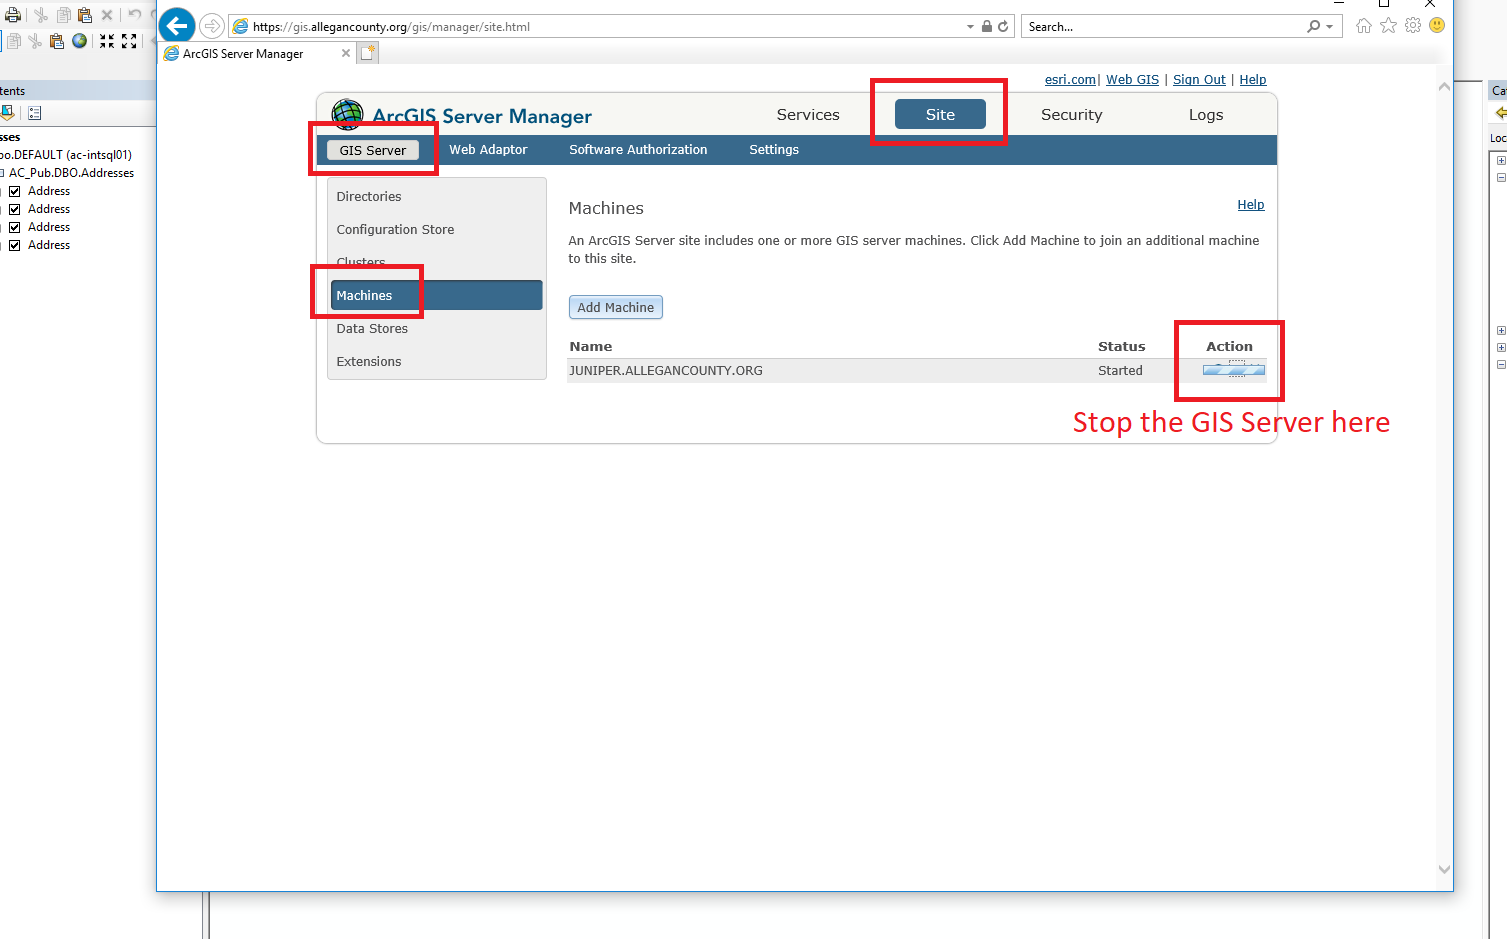
\includegraphics[width=.95\textwidth]{stopGisServer.png}
\caption{Stop the GIS Server}
\end{figure}
    %
\clearpage
    %
\subsubsection[Fixing Damaged Services]{Fixing Damaged Services\texorpdfstring{\\}{}}
    %
\paragraph*{Error: \texorpdfstring{\\}{}}
    %
\noindent \textbf{Service is currently being configured by another administrative operation}
    %
\paragraph*{Remedy: \texorpdfstring{\\}{}}
    %
\noindent This tech support article applies:\\
    %
\href{https://support.esri.com/en/technical-article/000015549}{https://support.esri.com/en/technical-article/000015549}
    %
\vspace{.25in}

\noindent There are at least 2 ways to fix:
    %
\begin{itemize}
    %
\item Use the ArcGIS Server Account Utility
    %
\item Remove Lock Files
    %
\end{itemize}
    %
\paragraph[Use the ArcGIS Server Account Utility]{Use the ArcGIS Server Account Utility\texorpdfstring{\\}{}}
    %
\subparagraph*{Access the GIS Server\texorpdfstring{\\}{}}
    %
\noindent To Log in to Juniper
    %
\vspace{.25in}

\noindent windows R $\Rightarrow$ mstsc
    %
\vspace{.25in}

\noindent $\Rightarrow$ juniper
    %
\vspace{.25in}

\noindent Use personal network credentials
    %
\clearpage
    %
\subparagraph*{On the GIS Server (Juniper)\texorpdfstring{\\}{}}
    %
\begin{wrapfigure}{r}{0.5\textwidth}
    %
\centering
    %
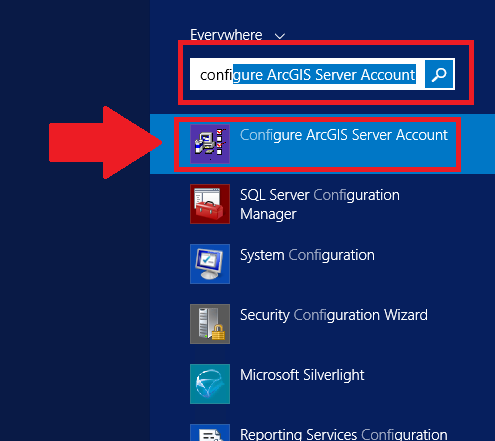
\includegraphics[width=.5\textwidth]{ArcGISServerAccountUtility.png}
    %
\caption{ArcGIS Server Accounty Utility}
    %
\vspace{.25in}
    %
\HRule \\[.4cm] % Horizontal Line added
    %
\vspace{.25in}

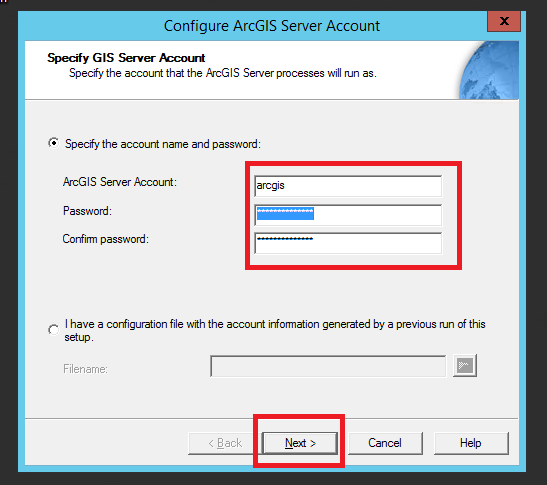
\includegraphics[width=.5\textwidth]{AccountUtilityLogin.PNG}
    %
\caption{Accounty Utility Login}
    %
\end{wrapfigure}
    %
\vspace{.5in}

In Windows Search, find:
    %
\vspace{.35in}

\noindent \textbf{Configure ArcGIS Server Account Utility}
    %
\vspace{3in}

\noindent Use credentials:
    %
\vspace{.35in}

\begin{verbatim}
PW:  @lleganGxxxxxx
\end{verbatim}
    %
\clearpage
    %
\noindent In the utility, paste these paths:
    %
\begin{verbatim}
C:\arcgisserver\directories
C:\arcgisserver\config-store
C:\arcgisserver\logs
\end{verbatim}
    %
\begin{figure}[h!]
    %
\centering
    %
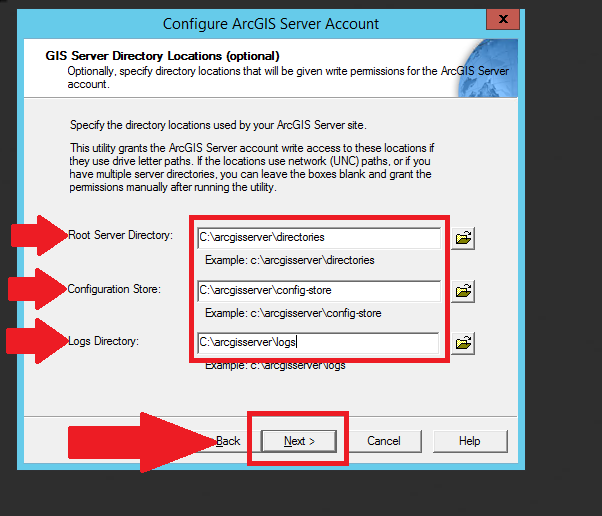
\includegraphics[width=.9\textwidth]{gisDirectoryLocationsFilled.png}
    %
\caption{GIS Directory Locations Filled}
    %
\end{figure}
    %
\noindent\textbf{\Large Push Next}
    %
\clearpage
    %
\noindent Select option \textbf{Do not export Configuration File}

\begin{figure}[h!]
    %
\centering
    %
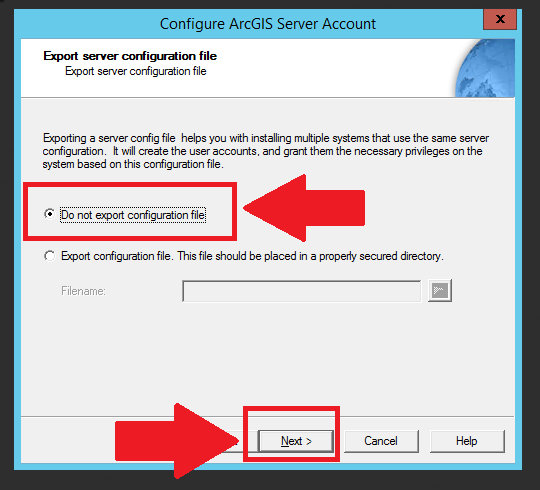
\includegraphics[width=.6\textwidth]{doNotExportConfigFile.PNG}
    %
\caption{Do not Export Config File}
    %
\end{figure}
    %
\noindent\textbf{\Large Push Next}
    %
%\subparagraph*{\texorpdfstring{\\}{}}
\subparagraph*{}
    %
\begin{figure}[h!]
    %
\centering
    %
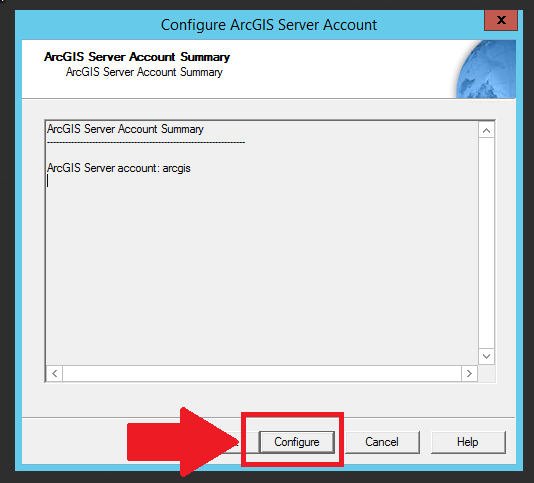
\includegraphics[width=.6\textwidth]{configureAccount.png}
    %
\caption{Configure Account}
    %
\end{figure}
    %
\noindent\textbf{\Large Push Configure}
    %
\clearpage
    %
\noindent While the tool runs, open the service manager\\
    %
\noindent In Windows Search, find:\\
    %
\textbf{Service Manger}
    %
\begin{figure}[h!]
\centering
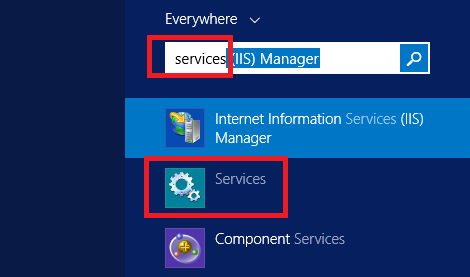
\includegraphics[width=.5\textwidth]{searchForServiceManager.PNG}
\caption{Search For Service Manager}
\end{figure}
    %
Launch \textbf{Service Manger}
    %
\vspace{.2in}
    %
\subparagraph*{\texorpdfstring{\\}{}}
    %
\noindent When the tool completes, \textbf{\Large Press Finish}
    %
\begin{figure}[h!]
\centering
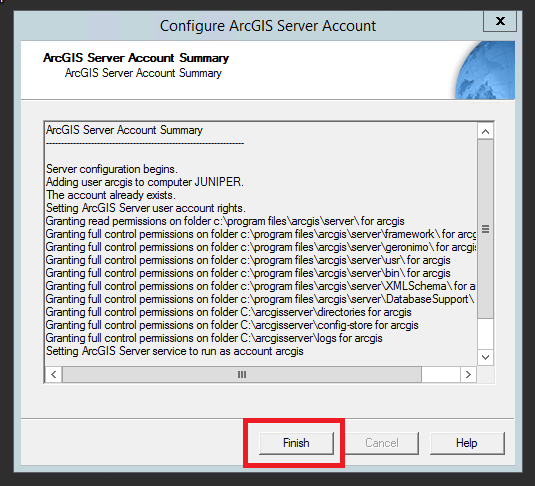
\includegraphics[width=.5\textwidth]{finishOnConfigure.png}
\caption{Finish On Configure}
\end{figure}
    %
\clearpage
    %
\subparagraph*{Services Manager}
    %
\begin{figure}[h!]
\centering
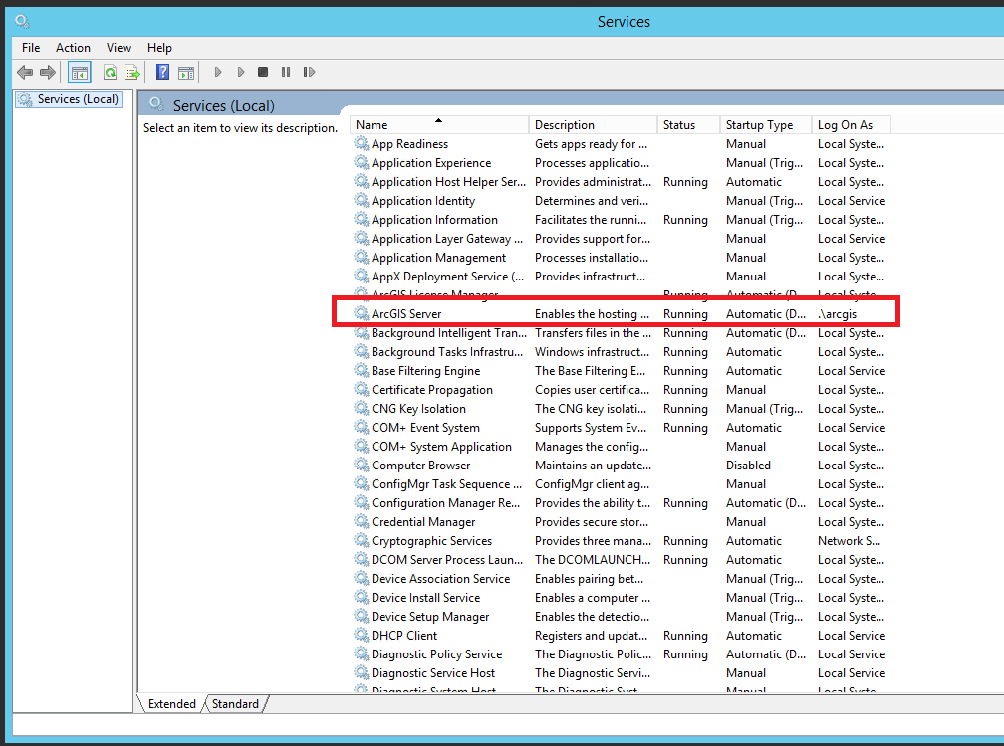
\includegraphics[width=.5\textwidth]{openServicesManager.png}
\caption{Open Services Manager}
\end{figure}
    %
\subparagraph*{}
    %
\noindent In services, select the ArcGIS Server service and restart the service.  (Randy had to do this)\\

\begin{figure}[h!]
\centering
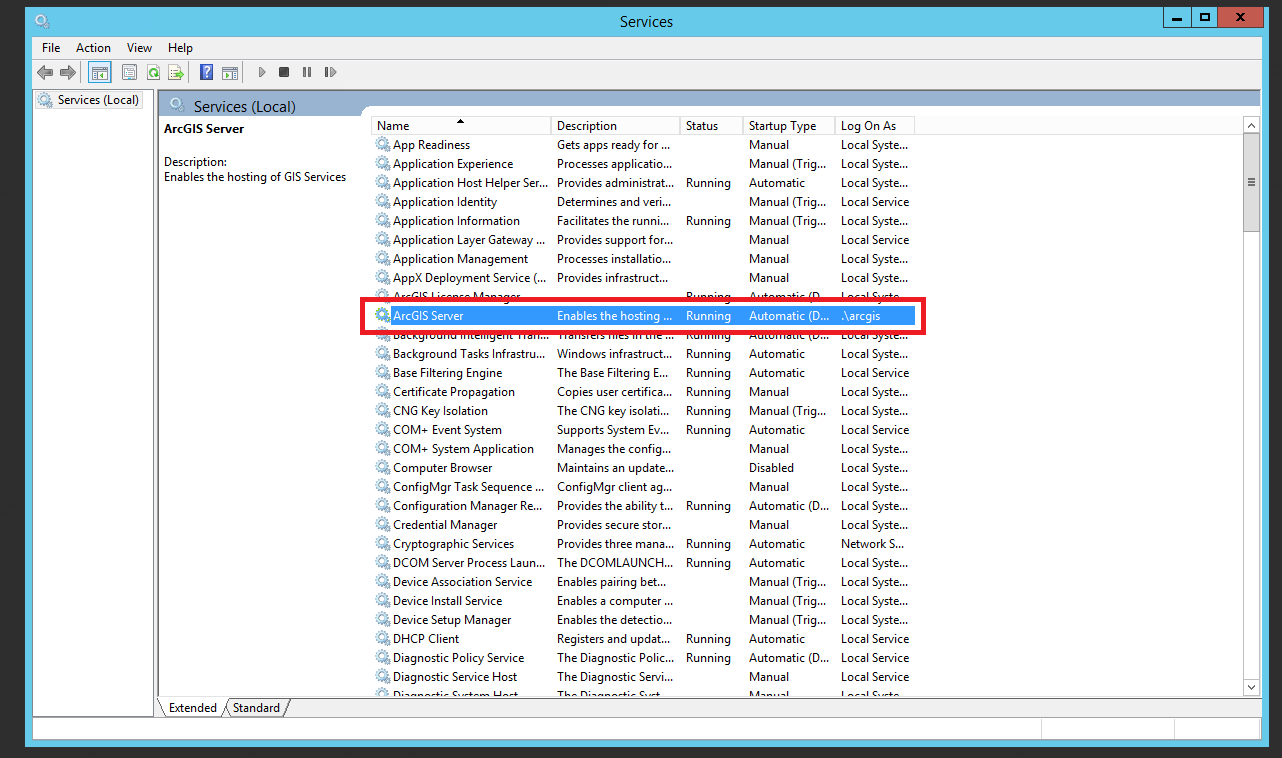
\includegraphics[width=.75\textwidth]{arcGisServiceInServicesManager.png}
\caption{arcGis Service In Services Manager}
\end{figure}


\clearpage


\paragraph*{Quick and dirty fix\texorpdfstring{\\}{}}

    %
\noindent When a service get hung up in som admin process, you may get an error like:
    %
\paragraph*{Error: \texorpdfstring{\\}{}}
    %
\noindent \textbf{Service is currently being configured by another administrative operation}
    %
\subparagraph[Remove Lock Files]{Removing Lock Files \texorpdfstring{\\}{}}
This may work, here is a blog about it\\
\href{https://community.esri.com/thread/103710}{https://community.esri.com/thread/103710}
Network location for an example service\\
\begin{verbatim}
on juniper
C:\arcgisserver\config-store\services\ParcelViewer2\
PV2Adresses.MapServer\startup\JUNIPER.ALLEGANCOUNTY.ORG

Suggested Steps:

1)stop arcgis server services.

2)delete the lock files(*.glock and *.rlock )
    (in arcgisserver\config-store).

3) restart arcgis server service.

4)stop the pending stopping service and then start it.
\end{verbatim}


mapservices would not stop so I try this:


\href{https://support.esri.com/en/technical-article/000012685}{https://support.esri.com/en/technical-article/000012685}


Check permission levels for the arcGIS account
ArcGisServerPermissions.PNG


If necessary, add the arcgis user to the permissions on the folders
ArcGisServerPermissionsAddUser.PNG


\end{document}
